\documentclass[a4paper]{article}

\usepackage[a4paper, top=8mm, bottom=8mm, left=8mm, right=8mm]{geometry}

\usepackage{polyglossia}
\setdefaultlanguage[babelshorthands=true]{russian}
\setotherlanguage{english}

\usepackage{fontspec}
\setmainfont{FreeSerif}
\newfontfamily{\russianfonttt}[Scale=0.7]{DejaVuSansMono}

\usepackage[tiny, compact]{titlesec}

\usepackage{titling}
\setlength{\droptitle}{-1cm}
\pretitle{\begin{center}\begin{bfseries}\Large}
\posttitle{\par\end{bfseries}\end{center}}
\preauthor{\begin{center}\normalsize}
\postauthor{\par\end{center}\vspace{-1.8cm}}

\usepackage{hyperref}
\usepackage{bookmark}
\usepackage{csquotes}
\usepackage{graphicx}

\title{Разработка драйвера камеры OV7670 для микроконтроллера МИК32}
\author{Гаврилов Максим Юрьевич}
\date{}

\begin{document}

\maketitle

\begin{flushright}
    Группа: \emph{\enquote{25.Б43-мм}}

    Кафедра: \emph{системного программирования}

    Научный руководитель: \emph{Пономарев Николай Алексеевич}
    
    Номер семестра практики: \emph{2}
\end{flushright}

\section{Введение}
Современные встраиваемые системы всё чаще включают в себя обработку визуальной информации: от систем безопасности до устройств интернета вещей.
Одной из самых доступных и распространённых камер для таких задач является OV7670 — недорогой CMOS-сенсор с разрешением до VGA.
В то же время российский рынок микроэлектроники активно развивается: микроконтроллеры с открытой архитектурой RISC-V, такие как МИК32 Амур ELBEAR ACE-UNO, становятся альтернативой зарубежным решениям.
Однако готовых и открытых, хорошо документированных драйверов для подключения камеры к этому контроллеру на момент 1 мая 2026 года не было, что затрудняло его применение в проектах, требующих получения и обработки изображений.

Разработка драйвера для камеры OV7670 под микроконтроллер МИК32 сопряжена с рядом технических трудностей:
нестандартный протокол управления SCCB, высокие требования к тактированию и скорости чтения кадров, ограниченный объём памяти.
В рамках данной работы предлагается изучить протокол SCCB, реализовать программный bit-bang для управления камерой без использования аппаратного I2C, оптимизировать код с учётом высоких требований к скорости выполнения и объёму памяти.

\section{Цель работы}
Исследование архитектуры RISC-V на примере микроконтроллера MIK32 Амур ELBEAR ACE-UNO и разработка низкоуровневого драйвера для камеры OV7670.

\section{Характеристики микроконтроллера}
В учебных целях был использован микроконтроллер 
\textbf{MIK32 Амур ELBEAR ACE-UNO} со следующими характеристиками:
\begin{itemize}
    \item максимальная рабочая частота 32 МГц
    \item объем встроенной памяти ОЗУ 16 КиБ
    \item объем встроенной памяти EEPROM 8 КиБ
    \item объём внешней Flash-памяти 2 ГБ
\end{itemize}

\section{Реализация}
\subsection{Выбор языка и библиотек}
Для написания прошивки был выбран язык \textbf{C}, так как он используется в HAL-библиотеках к микроконтроллеру МИК32.

В проекте использовались следующие сторонние пакеты:
\begin{itemize}
    \item \textbf{MIK32 HAL}~--- низкоуровневый слой для управления регистрами микроконтроллера
    \item \textbf{MIK32 HAL-shared}~--- общие утилиты (задержки, printf, работа с таймерами).
    \item \textbf{Adafruit OV7670}~--- взята за основу как референсная реализация, но её логика была существенно переработана и адаптирована под архитектуру MIK32 и требования по производительности.
\end{itemize}

\subsection{Расширяемая библиотека Adafruit OV7670}
Драйверов для видеокамеры OV7670 для микроконтроллера МИК32 не было найдено, но существовали аналоги: \textit{Arduino\_OV767X}, \textit{ov7670-no-ram-arduino-uno}, \textit{OV7670-ESP32}.
Библиотека \textit{Adafruit OV7670} оказалась пригодной для переиспользования.
Было предложено написать ядро драйвера под архитектуру МИК32, что включало в себя: настройка GPIO, UART, SCCB, генерации ШИМ-сигнала, также реализацию логики считывания кадра.
Список проблем, которые необходимо было решить при реализации данного проекта:
    
    \begin{enumerate}
        \item \textbf{Формирование тактового сигнала XCLK}

        OV7670 требует тактовый сигнал частотой от 10 до 48 МГц. При этом скорость выдачи кадров (кадров в секунду) оказывается высокой, что создаёт нагрузку на систему.

        \item \textbf{Необходимость хранения и отображения данных}

        Полный кадр даже при небольшом разрешении не помещается в ограниченную память, а для отладки требуется визуализировать получаемое изображение.

        \item \textbf{Проприетарный протокол SCCB}

        Камера общается по протоколу SCCB, который является разновидностью I2C, но требует обработки сигнала NACK. Аппаратный I2C-модуль MIK32 не поддерживает корректную работу с NACK, что делает стандартный обмен невозможным.


        \item \textbf{Ограничения по памяти и скорости}
        Маленький объём внутренней ОЗУ и относительно медленная внешняя Flash-память не позволяют просто разместить все данные в стандартных секциях.

        
        \item  \textbf{Получение изображения}
        Необходимо не только получить <<сырые>> данные изображения на микроконтроллере, но и передать их на другое устройство с дальнейшим выводом на экран.

    \end{enumerate}

\subsection{Предложенные и реализованные решения}
    \begin{itemize}
        \item Использован ШИМ-выход таймера MIK32 для генерации 16 МГц на выводе XCLK.
        \item Установлено минимальное рабочее разрешение 40×30 пикселей.
        \item Вывод сырых данных через UART на ПК с последующей визуализацией скриптом, написанном на языке Python.
        \item Реализована программная bit‑bang реализация I2C, полностью адаптированная под требования SCCB.
        \item Пины данных (D0–D7) подключены к порту ввода так, что после чтения регистра GPIO значения битов уже находятся на нужных позициях. Требуются только операции маскирования и сдвига, без перестановки битов.
        \item Критичные по скорости функции вынесены в RAM-память.
        \item Буфер для текущего обрабатываемого кадра размещён не в сегменте данных, а в стеке. Это обеспечило более эффективный доступ и меньшую фрагментацию.  
        \item Реализована передача <<сырых>> данных кадра с помощью UART на ПК, дальнейшая их обработка и получение изображения в формате \textit{.ppm}.
    \end{itemize}

    \subsubsection{Реализация тактового сигнала}
    Для реализации тактового сигнала был использован встроенный таймер, подключенный к внутреннему источнику тактирования, с возможностью генерации ШИМ сигнала со скважностью равной 50\%.
    В MIK32 есть несколько таймеров двух видов: TIMER32 и TIMER16, которые имеют 32-битный и 16-битный регистры для хранения счётчика соответственно.
    Каждый таймер имеет каналы, которые обладают своими особенными возможностями и характеристиками.
    Каждый канал подключен к выводу GPIO.
    Был выбран второй таймер TIMER16, так как в документации к MIK32 указано, что данный тип наиболее подходит для генерации тактового сигнала.
    Когда был подключен тактовый сигнал, можно было начинать общение с камерой.

    \subsubsection{Детали реализации bit‑bang SCCB}
    Хорошим выбором было бы использование аппаратного I2C, однако данный модуль в микроконтроллере МИК32 не поддерживает корректную обработку сигнала NACK. 
    При получении 9 бита информации периферийный блок отказывался принимать и отправлять данные. 
    Такое состояние можно было сбросить, послав сигнал STOP, однако он же и означал разрыв соединения с камерой.

    Была написана функция, реализующая bit-bang — метод программного управления линиями ввода-вывода (GPIO) для генерации сигналов протокола обмена данными.
    В данном случае линии SCL и SCL управляются вручную, что позволяет точно имитировать протокол I2C с учётом 9-го бита подтверждения.
    Это позволило корректно инициализировать регистры и наладить общение с камерой.

    \subsubsection{Оптимизация доступа к данным}
    Из-за того, что внешняя Flash-память работает медленно, выполнение кода из неё приводило к пропуску пикселей (разрывам изображения).
    Перенос функций, требующих высокой производительности, в RAM позволил увеличить скорость и достичь стабильной работы.


    \subsubsection{Оптимизация скорости чтения кадра}
    Изначально буфер с данными кадра хранился в области данных, однако была предпринята попытка перенести их в область стека.
    Данное решение позволило ускорить доступ к памяти и достичь более высокой производительности и стабильности чтения.

    \subsubsection{Вывод изображения}
    Был выбран протокол UART, так как он достаточно прост в использовании, обладает высокой скоростью, и для передачи данных нужно только 2 провода, не считая GND.
    Написан программный модуль, который реализует отправку данных кадра и отладочной информации.
    Далее был создан скрипт, написанный на языке Python с использованием библиотеки \textit{pyserial}, который считывает данные изображения и создаёт файл в расширении textit{.ppm}.

\subsection{Оптимизация работы с памятью}
\textit{Исполнение кода из внешней Flash-памяти.}
Самая низкая эффективность была зафиксирована при выполнении кода из внешней Flash, подключённой по интерфейсу SPIFI. 
Ограниченная пропускная способность этого интерфейса и дополнительные задержки при каждом обращении к шине приводили к тому, что процессор простаивал в ожидании очередной инструкции. 
Это вызывало пропуск пиксельных данных и, как следствие, разрывы изображения и потерю синхронизации.

\textit{Перенос ключевых функций в RAM.}
Перемещение функций, отвечающих за чтение пикселей и их первичную обработку, во внутреннюю SRAM кардинально изменило ситуацию~--- был получен стабильный захват кадра. 

\textit{Размещение буфера в сегменте данных \textit{vs.} в стеке.}
Размещение буфера кадра в стеке (как локальной переменной) оказалось эффективнее, чем в сегменте данных (глобальная переменная). 
Доступ к элементам стека часто требует более коротких инструкций (с использованием регистра \texttt{sp} и константного смещения). 

Таким образом, на практике подтверждён теоретический принцип: для задач реального времени критически важно минимизировать «расстояние» между процессором и исполняемым кодом/данными. 
Наиболее эффективными стратегиями в данном проекте оказались вынос функций обработки во внутреннюю RAM и размещение рабочих буферов в стеке.


\section{Тестирование}

\subsection{Получение изображения}
Были получены изображения (cм. рис. \ref{fig:test_image}, \ref{fig:realtime_image}) с камеры в разрешении 40х30.
Тестовые кадры в режимах \texttt{TEST\_PATTERN\_COLOR\_BAR} и \texttt{TEST\_PATTERN\_COLOR\_BAR\_FADE}, определенных в библиотеке Adafruit, оказались корректно отображены, однако в правой части экрана видны артефакты в виде <<лишней>> цветной линии, что связано с ошибкой в библиотечной реализации вывода изображения камеры в данном разрешении.

\begin{figure}[h]
\centering

\includegraphics[width=0.5\linewidth]{images/camera_image1.png}
\caption{Тестовое изображение, режим \texttt{TEST\_PATTERN\_COLOR\_BAR\_FADE}}
\label{fig:test_image}
\end{figure}

\begin{figure}[h]
\centering
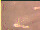
\includegraphics[width=0.5\linewidth]{images/camera_image2.png}
\caption{Изображение, получаемое с камеры в реальном времени}
\label{fig:realtime_image}
\end{figure}

Кадры, получаемые в реальном времени, некорректны.
При наведении камеры на тёмные места, изображение правильно, однако при её использовании на светлых участках видны белые пиксели.
Данная проблема может быть связана с ошибочной реализацией чтения кадра или с тем, микроконтроллер не успевает обработать приходящие данные.

\subsection{Достигнутая производительность}
\begin{itemize}
    \item Разрешение кадра в 40×30 пикселей.
    \item Достигнута стабильная частота 7 кадров в секунду.
\end{itemize}

\section{Заключение}
В ходе выполнения работы была совершена попытка разработки драйвера камеры OV7670 для микроконтроллера MIK32 Амур ELBEAR ACE-UNO (архитектура RISC-V).

\textbf{Выполненные задачи:}

    \begin{itemize}
        \item     Реализован bit-bang SCCB.
        \item     Реализована поддержка MIK32 в библиотеке Adafruit для камеры OV7670.
        \item     Получено изображение с камеры в тестовом режиме (cм. рис. \ref{fig:test_image}, \ref{fig:realtime_image}), однако испытываются проблемы при снятии кадра в реальном времени.
        \item     Достигнута частота 7 FPS при разрешении 40×30
    \end{itemize}

\begin{thebibliography}{99}
\bibitem{mik32} 
Техническое описание К1948ВК018, К1948ВК015 RISC-V микроконтроллер MIK32 АМУР(Версия 2.2.3)~--- URL: \url{https://docs.mikron.ru/wiki/_attachments/mik32_datasheet_v2_2_3.pdf} (дата обращения: 01.06.2026).

 \bibitem{sccb} 
 OmniVision Serial Camera Control Bus (SCCB)
Functional Specification~---  URL: \url{https://people.ece.cornell.edu/land/courses/ece4760/FinalProjects/f2021/jfw225_aei23_dsb298/jfw225_aei23_dsb298/SCCBSpec_AN.pdf} (дата обращения: 01.06.2026).

\bibitem{ov7670}
OV7670 datasheet~--- URL: \url{https://www.voti.nl/docs/OV7670.pdf} (дата обращения: 01.06.2026).

\bibitem{i2c}
Basics of the I2C Communication Protocol~--- URL: \url{https://www.circuitbasics.com/basics-of-the-i2c-communication-protocol/} (дата обращения: 01.06.2026).

\bibitem{github} 
 OV7670 driver for MIK32 ELBEAR ACE-UNO~--- URL: \url{https://github.com/energyc0/ov7670_mik32_driver} (дата обращения: 05.06.2026).
 
\end{thebibliography}

\end{document}